\section{Servlet}

\subsection{MVC Servlet 简介}

Spring MVC是Spring Framework提供的Web组件,全称是Spring Web MVC,是目前主流的实现MVC设计模式的框架,提供前端路由映射、视图解析等功能\footnote{这节参考文献: \url{https://blog.csdn.net/qq_52797170/article/details/125591705}}。

MVC是一种软件架构思想,把软件按照模型,视图,控制器来划分:
\begin{itemize}
    \item 模型(Model): 指工程中的JavaBean,用来处理数据。JavaBean分成两类:
    \begin{itemize}
        \item 实体类Bean: 专门用来存储业务数据,比如Student,User。
        \item 业务处理Bean: 指Servlet或Dao对象,专门用来处理业务逻和数据访问。
    \end{itemize}
    \item 视图(View): 指工程中的html,jsp等页面,作用是和用户进行交互,展示数据
    \item 控制(Controller): 指工程中的Servlet,作用是接收请求和响应浏览器
\end{itemize}

\begin{figure}[H]
    \small
    \centering
    \begin{tikzpicture}[scale = 1]
        \node [draw] (0) at (0,0) {浏览器};
        \node [draw] (1) at (3,0) {Controller};
        \node [draw] (2) at (3,-1) {View};
        \node [draw] (3) at (6,0) {Model(Bean)};
        \node [draw] (4) at (9,0) {DB};
        \draw[-Stealth] (0) -- (1) node [midway,above,font=\footnotesize] {请求};
        \draw[-Stealth] (2) -- (0) node [midway,below,font=\footnotesize] {响应};
        \draw[-Stealth] (1) -- (2);
        \draw[Stealth-Stealth] (1) -- (3);
        \draw[Stealth-Stealth] (3) -- (4);
    \end{tikzpicture}
    \caption{MVC 设计模式}
    \label{fig:MVC 设计模式}
\end{figure}

Spring MVC 包含以下核心组件:
\begin{itemize}
    \item DispatcherServlet: 前端控制器,负责调度其他组件的执行,可以降低不同组件之间的耦合性,是整个Spring MVC的核心模块
    \item Handler: 处理器,完成具体的业务逻辑,相当于 Servlet。
    \item HandlerMapping: DispatcherServlet 通过它把请求映射到不同的 Handler。
    \item HandlerInterceptor: 处理拦截器,用于进行一些拦截处理,是一个接口。
    \item HandlerExecutionChain: 处理器执行链,包括两部分内容:Handler和HandlerInterceptor。
    \item HandlerAdapter: 处理器适配器,Handler执行业务方法之前,需要进行一系列的操作。
    \item ModelAndView: 封装了模型数据和视图信息,作为Handler的处理结果,返回给DispatcherServlet。
    \item ViewResolver:视图解析器,DispatcherServlet通过它把逻辑视图解析为物理视图,最终把渲染的结果响应给客户端。
\end{itemize}

\begin{figure}[H]
    \centering
    \begin{tikzpicture}[scale = 1]
        \node [draw] (client) at (0,0) {客户端};
        \node [draw] (dispatch) at (5,0) {DispatcherServlet};
        \node [draw] (map) at (12,0) {HandlerMapping};
        \node [draw] (view) at (2,-3) {ViewResolver};
        \node [draw] (adapter) at (7,-3) {HandlerAdapter};
        \node [draw] (handler) at (12,-3) {Handler};
        \begin{scope}[font = \scriptsize]
            \draw [-Stealth] ([yshift=4pt]client.east) -- ([yshift=4pt]dispatch.west) node [midway, above] {request};
            \draw [-Stealth] ([yshift=-4pt]dispatch.west) -- ([yshift=-4pt]client.east) node [midway, below] {response};
            \draw [-Stealth] ([yshift=4pt]dispatch.east) -- ([yshift=4pt]map.west) node [midway, above] {获取 Handler};
            \draw [-Stealth] ([yshift=-4pt]map.west) -- ([yshift=-4pt]dispatch.east) node [midway, below] {返回 HandlerExecutionChain};
            \draw [-Stealth] ([xshift=-20pt]dispatch.south) -- ([xshift=-4pt]view.north) node [midway, left] {解析 ModelAndView};
            \draw [-Stealth] ([xshift=4pt]view.north) -- ([xshift=-12pt]dispatch.south) node [midway, right] {返回 View};
            \draw [-Stealth] ([xshift=12pt]dispatch.south) -- ([xshift=-4pt]adapter.north) node [midway, left] {};
            \draw [-Stealth] ([xshift=4pt]adapter.north) -- ([xshift=20pt]dispatch.south) node [midway, right] {返回 ModelAndView};
            \draw [-Stealth] ([yshift=4pt]adapter.east) -- ([yshift=4pt]handler.west) node [midway, above] {执行 Handler};
            \draw [-Stealth] ([yshift=-4pt]handler.west) -- ([yshift=-4pt]adapter.east) node [midway, below] {返回 ModelAndView};
        \end{scope}
    \end{tikzpicture}
    \caption{MVC 工作流程}
    \label{fig:MVC 工作流程}
\end{figure}

假设有下面代码,分析其工作流程:
\begin{Java}
@Controller
public class HelloHandler {
    @RequestMapping("/index")
    public String index() {
        System.out.println("接收到 index 请求");
        return "index";
    }
}
\end{Java}

此时 SpringMVC 的处理流程如下:

\begin{itemize}
    \item 客户端尝试获取 “/index” 页面时
    \item DispatcherServlet 接收到 URL 请求 index,尝试通过 HandlerMapping 获取对应的 Handler
    \item 结合 @RequestMapping,HandlerMapping 返回 HelloHandler。
    \item 调用 HelloHandler 中对应的方法,返回 ``index'' 字符串。
    \item ViewResolver 解析 ``index'' 字符串,找到目标资源: /index.html(也可能是其他类型的资源,如 jsp) 并将该资源返回。
\end{itemize}

这段代码实际中的响应过程如下:

\begin{figure}[H]
    \centering
    \begin{tikzpicture}[scale = 1]
        \node [draw] (client) at (0,0) {客户端};
        \node [draw] (dispatch) at (5,0) {DispatcherServlet};
        \node [draw] (map) at (12,0) {HandlerMapping};
        \node [draw] (view) at (2,-3) {ViewResolver};
        \node [draw] (adapter) at (7,-3) {HandlerAdapter};
        \node [draw] (handler) at (12,-3) {Handler};
        \begin{scope}[font = \scriptsize]
            \draw [-Stealth, red] ([yshift=4pt]client.east) -- ([yshift=4pt]dispatch.west) node [midway, above, black] {1: Get ``index''};
            \draw [-Stealth, orange] ([yshift=-4pt]dispatch.west) -- ([yshift=-4pt]client.east) node [midway, below, black] {10: 返回 index.html};
            \draw [-Stealth, red] ([yshift=4pt]dispatch.east) -- ([yshift=4pt]map.west) node [midway, above, black] {2: 获取对应 Handler};
            \draw [-Stealth, red] ([yshift=-4pt]map.west) -- ([yshift=-4pt]dispatch.east) node [midway, below, black] {3: 返回 index()};
            \draw [-Stealth, orange] ([xshift=-20pt]dispatch.south) -- ([xshift=-4pt]view.north) node [midway, left, black] {8: 解析 ModelAndView};
            \draw [-Stealth, orange] ([xshift=4pt]view.north) -- ([xshift=-12pt]dispatch.south) node [midway, right, black] {9: 返回 View};
            \draw [-Stealth, blue] ([xshift=12pt]dispatch.south) -- ([xshift=-4pt]adapter.north) node [midway, left, black] {4: 处理};
            \draw [-Stealth, blue] ([xshift=4pt]adapter.north) -- ([xshift=20pt]dispatch.south) node [midway, right, black] {7: 返回 ModelAndView};
            \draw [-Stealth, blue] ([yshift=4pt]adapter.east) -- ([yshift=4pt]handler.west) node [midway, above, black] {5. 执行对应 Handler};
            \draw [-Stealth, blue] ([yshift=-4pt]handler.west) -- ([yshift=-4pt]adapter.east) node [midway, below, black] {6: 返回 ModelAndView};
        \end{scope}
    \end{tikzpicture}
    \caption{例子工作流程}
    \label{fig:例子工作流程}
\end{figure}

\subsection{MVC Servlet 整体结构}

DispatcherServlet 的继承结构如下,其中 HttpServlet 为 Java 实现,其他为 Spring 内容。

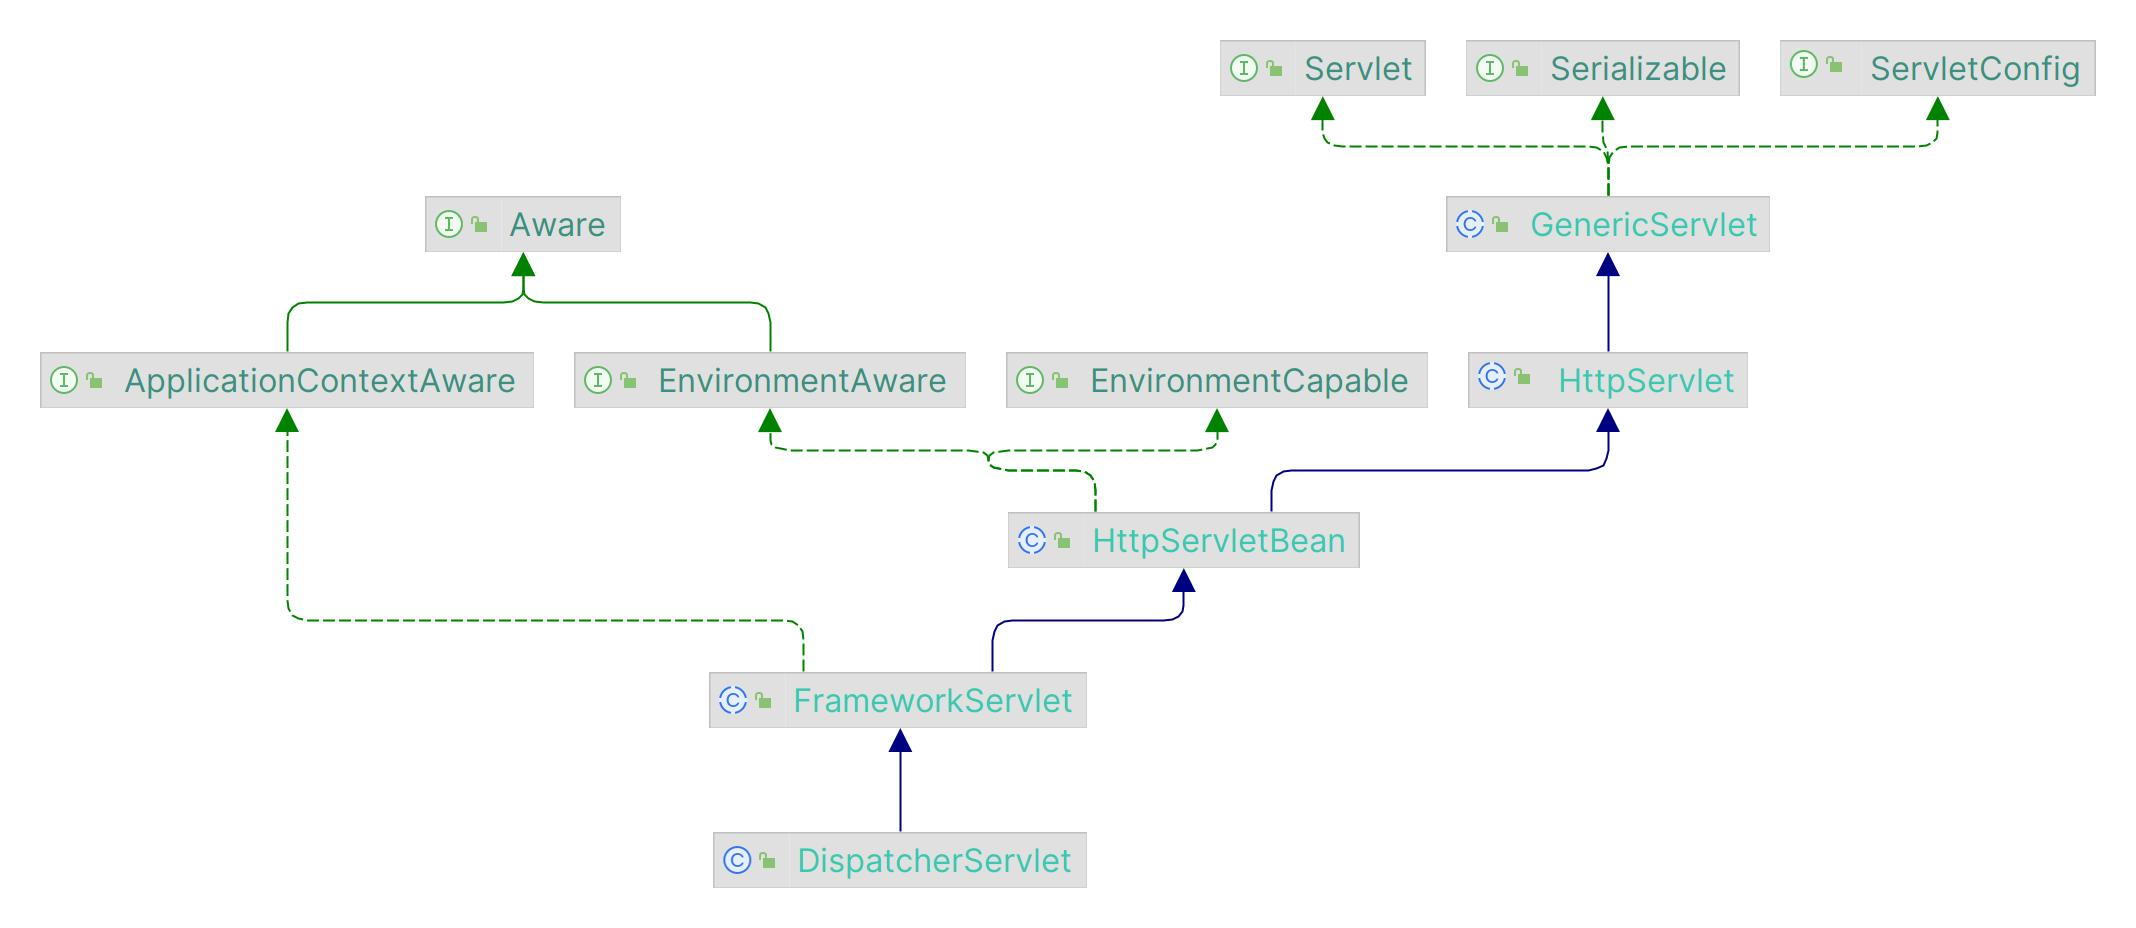
\includegraphics[width=0.9\linewidth]{../../../imgs/uml/DispatcherServlet.jpg}

\subsubsection{HttpServlet}

Servlet是Server + Applet的缩写,表示一个服务器应用。Java 中最基础的 Servlet 接口有如下规范:

\begin{Java}
public interface Servlet {
    void init(ServletConfig var1) throws ServletException;
    ServletConfig getServletConfig();
    void service(ServletRequest var1, ServletResponse var2) throws ServletException, IOException;
    String getServletInfo();
    void destroy();
}
\end{Java}

其中,init 与 destroy 分别在容器启动和销毁时调用,这两个方法都只会被调用一次。getServletConfig方法用于获取ServletConfig,getServletInfo方法可以获取一些Servlet相关的信息,如作者、版权等,这个方法需要自己实现,默认返回空字符串。

比较重要的 service方法用于具体处理一个请求; 是 Servlet 的主要功能。

Init方法被调用时会接收到一个ServletConfig类型的参数,是容器传进去的。配置一般来源于 xml 文件。 ServletConfig 接口定义如下:

\begin{Java}
public interface ServletConfig {
    public String getServletName();
    public ServletContext getServletContext();
    public String getInitParameter(String name);
    public Enumeration<String> getInitParameterNames();
}
\end{Java}

这几个方法都比较简单,必要重要的 getServletContext 返回值ServletContext代表的是我们这个应用本身。既然ServletContext代表应用本身,那么ServletContext里边设置的参数就可以被当前应用的所有Servlet共享了。我们做项目的时候都知道参数可以保存在Session中,也可以保存在Application中,而后者很多时候就是保存在了ServletContext中。

我们可以这么理解,ServletConfig是Servlet级的,而ServletContext是Context(也就是Application)级的。当然,ServletContext的功能要强大很多,并不只是保存一下配置参数,否则就叫ServletContextConfig了。

GenericServlet是Servlet的默认实现,源码非常简单不贴了,主要做了三件事:

\begin{itemize}
    \item 实现了ServletConfig接口,我们可以直接调用 ServletConfig 里面的方法;
    \item 提供了无参的init方法;
    \item 提供了log方法,可以记录日志或异常。
\end{itemize}

HttpServlet是用HTTP协议实现的Servlet的基类,写Servlet时直接继承它就可以了,不需要再从头实现Servlet接口。

既然HttpServlet是跟协议相关的,当然主要关心的是如何处理请求了,所以HttpServlet主要重写了service方法。在service方法中首先将ServletRequest和ServletResponse转换为了HttpServletRequest和HttpServletResponse,然后根据Http请求的类型不同将请求路由到了不同的处理方法。

具体的处理方法是 doXXX 结构 (doGet, doHead)。doGet, doPost, doPut, doDelete 方法都是模板方法,需要子类实现,否额会抛异常。
\begin{itemize}
    \item \textbf{doGet}: 针对 Get 方法做了优化,调用前会做过期检查,如果没有过期则直接返回304状态码使用缓存。
    \item \textbf{doHead}: 调用 deGet 方法,返回空 body 的 Response。
    \item \textbf{doOptions, doTrace}: 功能非常固定,HttpServlet 提供了默认实现。
\end{itemize}

\subsubsection{HttpServletBean}

在 DispatcherServlet 集成结构中,HttpServletBean 直接继承了 HttpServlet,同时实现了 EnvironmentCapable 和 EnvironmentAware 接口。首先我们需要知道有 Aware 和 Capable 后缀接口的意义:

\begin{itemize}
    \item Aware: Aware 接口本身是一个标识接口,XXXAware 在 spring 里表示对 XXX 可感知,如果在某个类里面想要使用 spring 的一些东西,就可以通过实现 XXXAware 接口告诉 spring 给你送过来,而接收的方式是通过实现接口唯一的方法 set-XXX。
    \item Capable: 具备某些能力,如具有 Environment 的能力, 当spring需要Environment的时候就会调用其getEnvironment方法跟它要。
\end{itemize}

Environment 是环境的意思,具体功能和 ServletContext 类似。在HttpServletBean中Environment使用的是Standard-Servlet-Environment,它封装了ServletContext,同时还封装了ServletConfig、JndiProperty、系统环境变量和系统属性,这些都封装到了其propertySources属性下。总而言之,很多环境相关的配置都存放在了 Environment 中。

在HttpServletBean的init中,首先将Servlet中配置的参数使用BeanWrapper设置到DispatcherServle的相关属性,然后调用模板方法initServletBean,子类就通过这个方法初始化。

\subsubsection{FrameworkServlet}

FrameworkServlet 实现了 ApplicationContextAware, 也即获得了获取 ApplicationContext 的能力。

Framework 实现了 initServletBean 方法,其中有两句核心代码:
\begin{Java}
this.webApplicationContext = initWebApplicationContext();
initFrameworkServlet();
\end{Java}

initFrameworkServlet方法是模板方法,子类可以覆盖然后在里面做一些初始化的工作。FrameworkServlet在构建的过程中的主要作用就是初始化了WebApplicationContext。initWebApplicationContext方法做了三件事:

\begin{itemize}
    \item 获取spring的根容器rootContext。
    \item 设置webApplicationContext并根据情况调用onRefresh方法。
    \item 将webApplicationContext设置到ServletContext中。
\end{itemize}

\subsubsection{DispathchServlet}

onRefresh方法是DispatcherServlet的入口方法。onRefresh中简单地调用了initStrategies,在initStrategies中调用了9个初始化方法:

\begin{Java}
@Override
protected void onRefresh(ApplicationContext context) {
	initStrategies(context);
}

protected void initStrategies(ApplicationContext context) {
	initMultipartResolver(context);
	initLocaleResolver(context);
	initThemeResolver(context);
	initHandlerMappings(context);
	initHandlerAdapters(context);
	initHandlerExceptionResolvers(context);
	initRequestToViewNameTranslator(context);
	initViewResolvers(context);
	initFlashMapManager(context);
}
\end{Java}

initStrategies的具体内容非常简单,就是初始化的9个组件。下面看一下 initLocaleResolver 的具体实现:

\begin{Java}
private void initLocaleResolver(ApplicationContext context) {
	try {
		this.localeResolver = context.getBean(LOCALE_RESOLVER_BEAN_NAME, LocaleResolver.class);
		if (logger.isTraceEnabled()) {
			logger.trace("Detected " + this.localeResolver);
		}
		else if (logger.isDebugEnabled()) {
			logger.debug("Detected " + this.localeResolver.getClass().getSimpleName());
		}
	}
	catch (NoSuchBeanDefinitionException ex) {
		// We need to use the default.
		this.localeResolver = getDefaultStrategy(context, LocaleResolver.class);
		if (logger.isTraceEnabled()) {
			logger.trace("No LocaleResolver '" + LOCALE_RESOLVER_BEAN_NAME +
					"': using default [" + this.localeResolver.getClass().getSimpleName() + "]");
		}
	}
}
\end{Java}

初始化方式分两步:首先通过context.getBean在容器里面按注册时的名称或类型(这里指“localeResolver”名称或者LocaleResolver.class类型)进行查找,如果找不到就调用getDefaultStrategy按照类型获取默认的组件。

\subsection{MVC Servlet 处理过程}

\subsubsection{FrameworkServlet}

前面讲过 Servlet 的处理过程:首先是从Servlet接口的 service 方法开始,然后在 Http-Servlet 的 service 方法中根据请求的类型不同将请求路由到了对应的 doXXX 方法中。

在FrameworkServlet中重写了service与大部分doXXX方法,(doHead 没重写)。在service方法中增加了对PATCH类型请求的处理,其他类型的请求直接交给了父类进行处理; 其中:
\begin{itemize}
    \item doOptions和doTrace方法可以通过设置dispatchOptionsRequest和dispatchTraceRequest参数决定是自己处理还是交给父类处理(默认都是交给父类处理,doOptions会在父类的处理结果中增加PATCH类型);
    \item doGet、doPost、doPut和doDelete都是自己处理。所有需要自己处理的请求都交给了processRequest方法进行统一处理。
\end{itemize}

\begin{Java}
@Override
protected void service(HttpServletRequest request, HttpServletResponse response) throws ServletException, IOException {
    HttpMethod httpMethod = HttpMethod.resolve(request.getMethod());
    if (httpMethod == HttpMethod.PATCH || httpMethod == null) {
        processRequest(request, response);
    }
    else {
        super.service(request, response);
    }
}

@Override
protected final void doGet(HttpServletRequest request, HttpServletResponse response)
        throws ServletException, IOException {
    processRequest(request, response);
}
\end{Java}

看到这可能会比较迷惑,为什么 service 调用父类 service 方法处理 request,又要自己重写 doXXX 方法,直接覆盖了service不是就可以了吗?原书的解释如下:

\fbox{
    \parbox{0.87\textwidth}{
        \begin{problem}
            可能有的读者会想,直接覆盖了service不是就可以了吗?HttpServlet是在service方法中将请求路由到不同的方法的,如果在service中不再调用super.service(),而是直接将请求交给processRequest处理不是更简单吗?从现在的结构来看确实如此,不过那么做其实存在着一些问题。比如,我们为了某种特殊需求需要在Post请求处理前对request做一些处理,这时可能会新建一个继承自DispatcherServlet的类,然后覆盖doPost方法,在里面先对request做处理,然后再调用supper.doPost(),但是父类根本就没调用doPost,所以这时候就会出问题了。虽然这个问题的解决方法也很简单,但是按正常的逻辑,调用doPost应该可以完成才合理,而且一般情况下开发者并不需要对Spring MVC内部的结构非常了解,所以Spring MVC的这种做法虽然看起来有点笨拙但是是必要的。
        \end{problem}
    }
}

那么,为什么自己处理的 doXXX 方法又要统一到 processRequest 中处理。下面看一下最核心的方法: processRequest。

processRequest方法中的核心语句是doService(request,response),这是一个模板方法,在DispatcherServlet中具体实现。在doService前后还做了一些事情(装饰器模式?),配置了一些信息做了一些判断。具体是如何实现的讲起来比较复杂,请看原文或者源码。

\subsubsection{DispatcherServlet}

通过之前的分析我们知道,DispatcherServlet里面执行处理的入口方法应该是doService,不过doService并没有直接进行处理,而是交给了doDispatch进行具体的处理,在doDispatch处理前doService做了一些事情: 首先判断是不是include请求,如果是则对request的Attribute做个快照备份,等doDispatch处理完之后进行还原。在做完快照后又对request设置了一些属性。比较复杂,看懂了再回来写。

doDispatch方法非常简洁,从顶层设计了整个请求处理的过程。doDispatch中最核心的代码只要4句,它们的任务分别是:

\begin{itemize}
    \item 根据 request 找到 Handler。
    \item 根据 Handler 找到对应的 HandlerAdapter。
    \item 用 HandlerAdapter 处理 Handler。
    \item 调用 processDispatchResult 方法处理上面处理之后的结果(包裹找到 View 并渲染输出给用户)。
\end{itemize}

\begin{Java}
mappedHandler = getHandler(processedRequest);
HandlerAdapter ha = getHandlerAdapter(mappedHandler.getHandler());
mv = ha.handle(processedRequest, response, mappedHandler.getHandler());
processDispatchResult(processedRequest, response, mappedHandler, mv, dispatchException);
\end{Java}

先解释三个概念: HandlerMapping、Handler和HandlerAdapter:
\begin{itemize}
    \item Handler: 处理器,直接对应 MVC 中的 Controller 层,具体表现形式有很多,可以是类,方法。@RequestMapping的所有方法都可以看成一个Handler。只要可以实际处理请求就可以是Handler。
    \item HandlerMapping: 是用来查找Handler的。
    \item HandlerAdapter: 因为Spring MVC中的Handler可以是任意的形式,只要能处理请求就OK,但是Servlet需要的处理方法的结构却是固定的,都是以request和response为参数的方法(如doService方法)。HandlerAdapter 负责进行适配,是最复杂的组件。
\end{itemize}

另外View和ViewResolver的原理与Handler和HandlerMapping的原理类似。View是用来展示数据的,而ViewResolver用来查找View。View里面的内容就是Model。

\subsubsection{doDispatch 结构}

doDispatch 大体可分为两部分: 处理请求(Handler)和渲染页面(View)。大致的实现逻辑如下:
\begin{itemize}
    \item 检查是不是上传请求,如果是上传请求,则将request转换为MultipartHttpServletRequest,并将multipartRequestParsed标志设置为true。其中使用到了MultipartResolver。
    \item 通过getHandler方法获取Handler处理器链,其中使用到了HandlerMapping,返回值为HandlerExecutionChain类型,其中包含着与当前request相匹配的Interceptor和Handler。
    \item 接下来是处理GET、HEAD请求的Last-Modified。浏览器第一次请求资源(GET、Head请求)时,返回的请求头里面会包含一个Last-Modified的属性,在浏览器以后发送请求时会同时发送之前接收到的Last-Modified,服务器接收到带Last-Modified的请求后会用其值和自己实际资源的最后修改时间做对比,判断是否需要更新。
    \item 接下来依次调用相应Interceptor的preHandle。
    \item 处理完成后,让HandlerAdapter使用Handler处理请求,Controller就是在这个地方执行的。这里主要使用了HandlerAdapter。
    \item Handler处理完请求后,如果需要异步处理,则直接返回,如果不需要异步处理,当view为空时(如Handler返回值为void),设置默认view,然后执行相应Interceptor的postHandle。设置默认view的过程中使用到了ViewNameTranslator。
    \item 到这里请求处理的内容就完成了,接下来使用processDispatchResult方法处理前面返回的结果,其中包括处理异常、渲染页面、触发Interceptor的afterCompletion方法三部分内容。
\end{itemize}

doDispatch 方法的具体实现比较复杂,涉及到很多组件,现在知道他是干什么的就行了。

\begin{figure}[H]
    \centering
    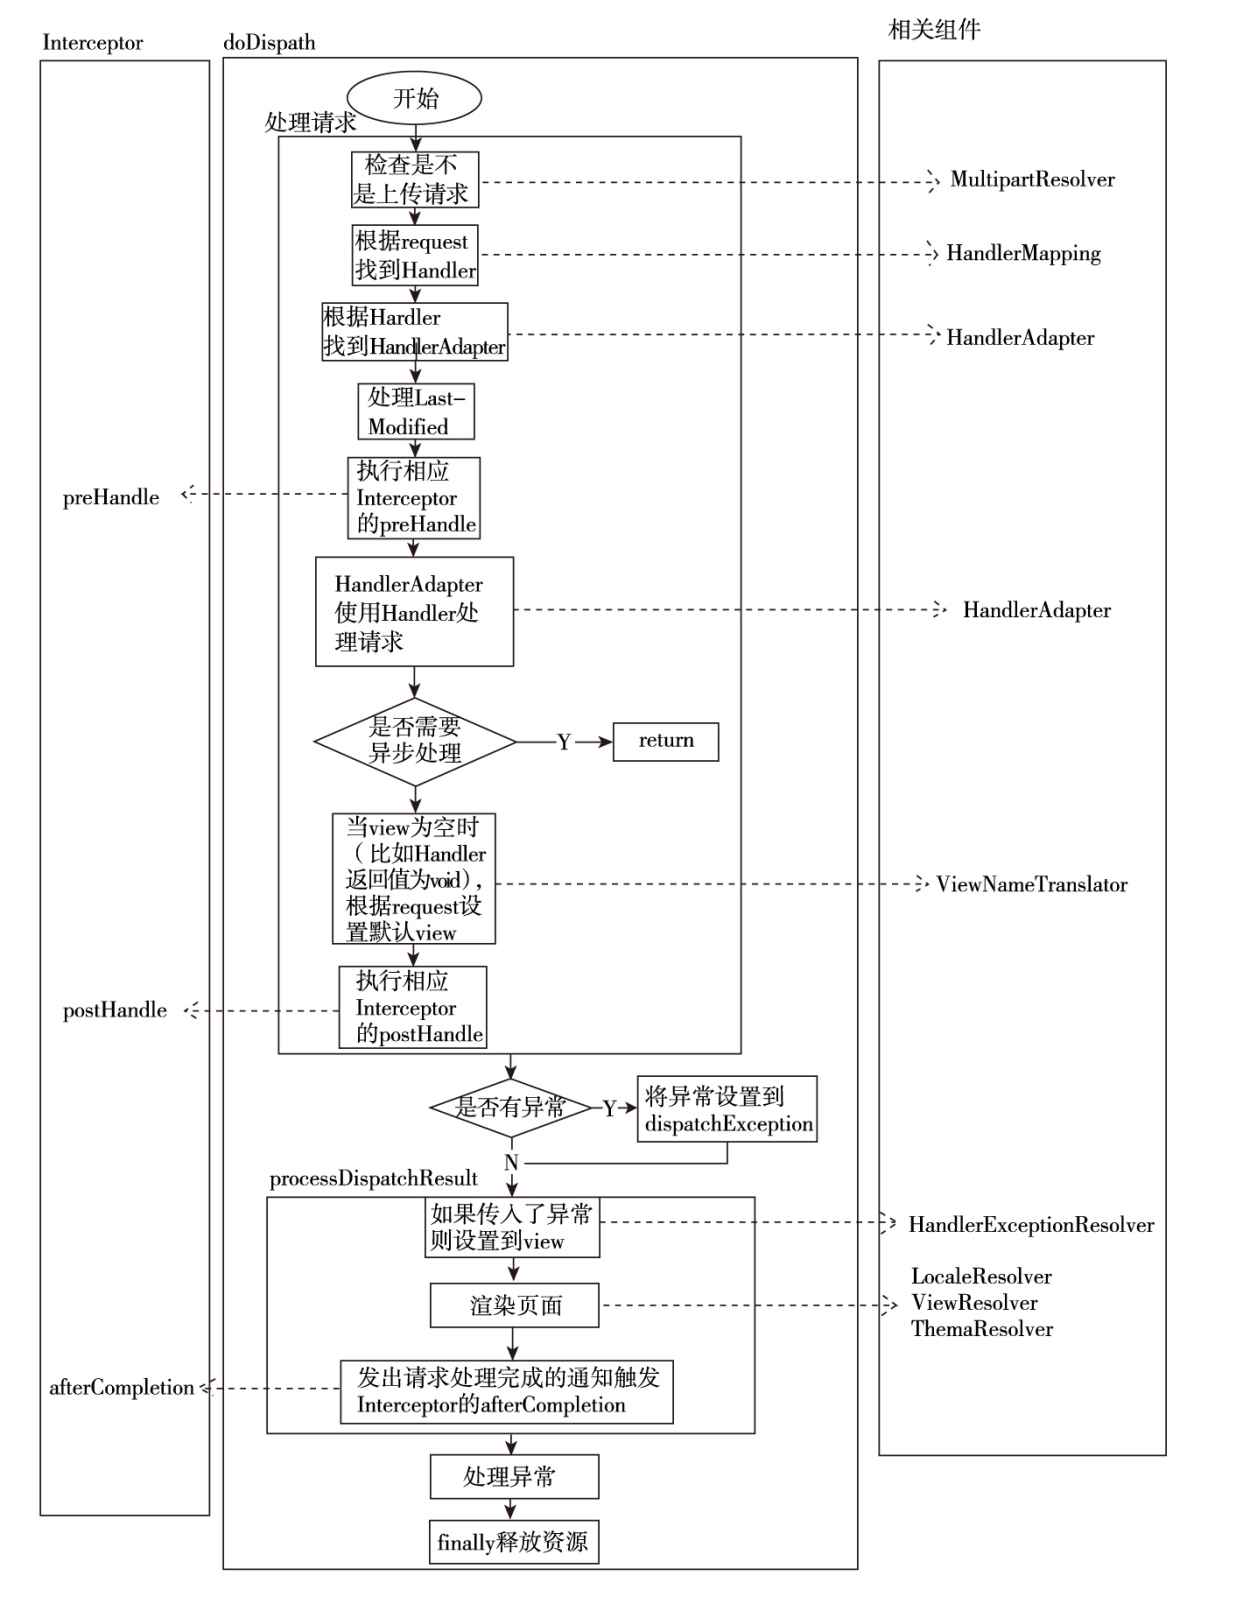
\includegraphics[width=0.9\linewidth]{../../../imgs/uml/doDispatch.png}
    \caption{doDispatch 方法处理流程(源自:<<看透 Spring MVC: 源代码分析与实践>>)}
    \label{fig:doDispatch 方法处理流程}
\end{figure}


\newpage